\section{Experiments}
\begin{figure*}[hbt]
    \centering
    \begin{subfigure}{0.49\textwidth}
        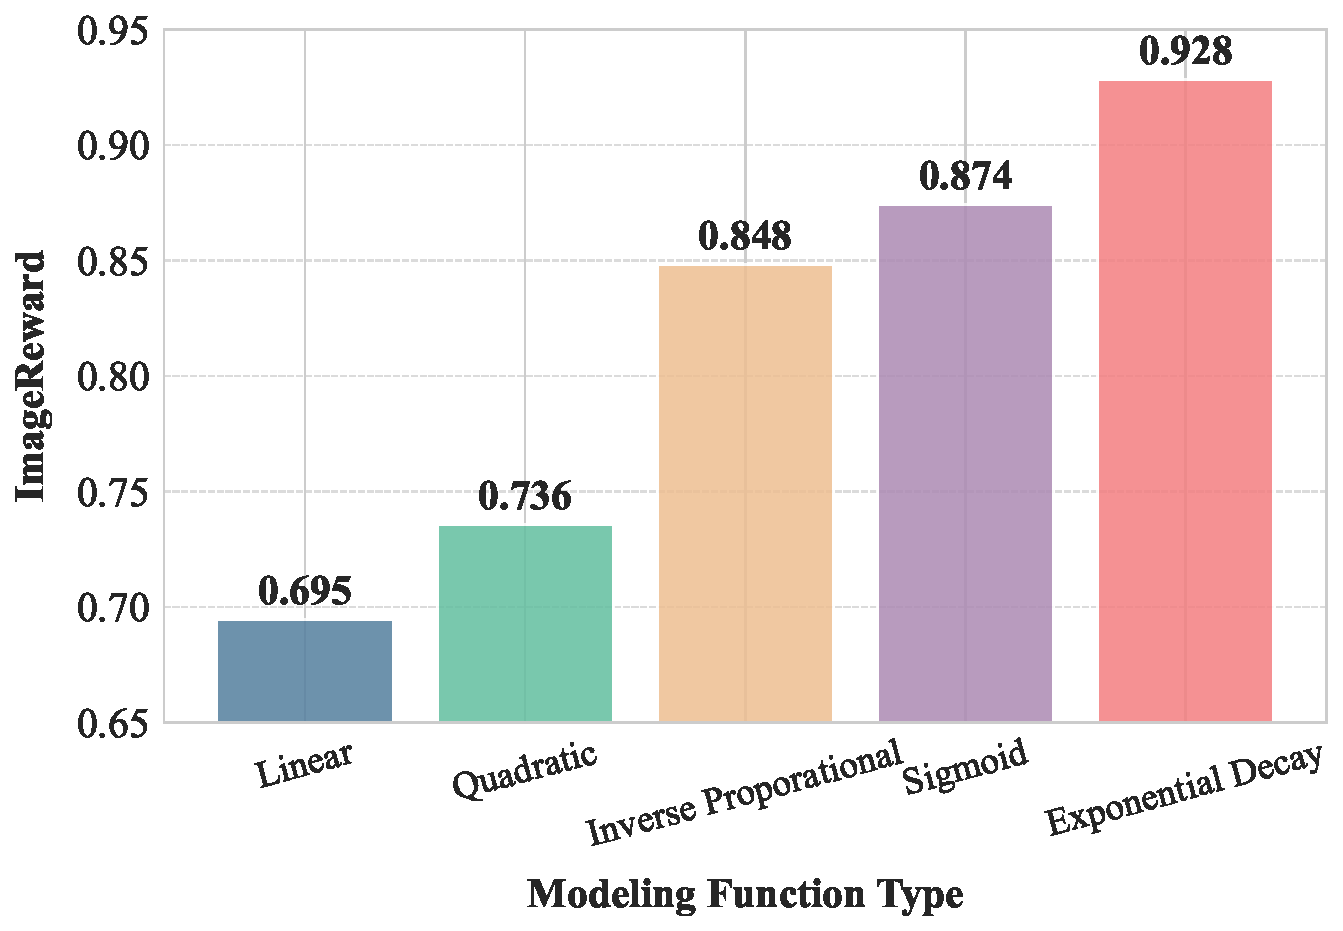
\includegraphics[width=\linewidth]{fig_tab/function_comparison_ImageReward.pdf}
        \captionsetup{justification=justified, singlelinecheck=true}
        \caption{Modeling function comparison: ImageReward.}
        \label{fig:sub1}
    \end{subfigure}
    \hfill
    \begin{subfigure}{0.49\textwidth}
        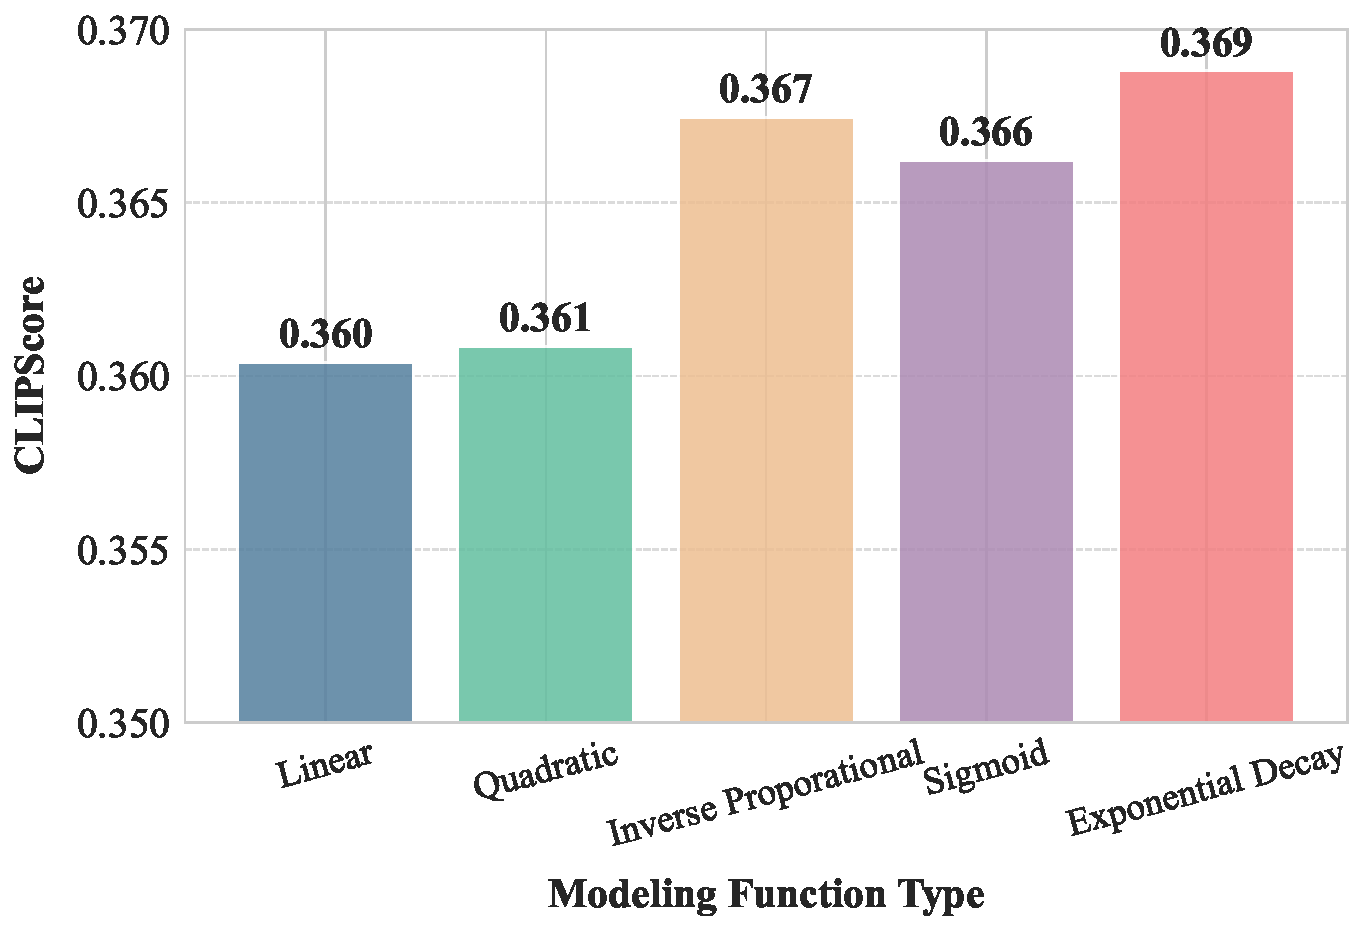
\includegraphics[width=\linewidth]{fig_tab/function_comparison_CLIPScore.pdf}
        \captionsetup{justification=justified, singlelinecheck=true}
        \caption{Modeling function comparison: CLIPScore.}
        \label{fig:sub2}
    \end{subfigure}
    \captionsetup{justification=justified, singlelinecheck=false}
    \caption{\textbf{Ablation studies on different types of modeling functions.} The comparative results demonstrate that the exponential decay function delivers the optimal fitting results among other functions, validating the soundness of our method.}
    \label{fig:function_ablation}
\end{figure*}
We evaluate \mtdbk on image and video generation, testing its effectiveness across architectures. We also study how design choices and hyperparameters affect performance.
% \begin{figure*}[t]
%     \centering
%     \begin{subfigure}{0.49\textwidth}
%         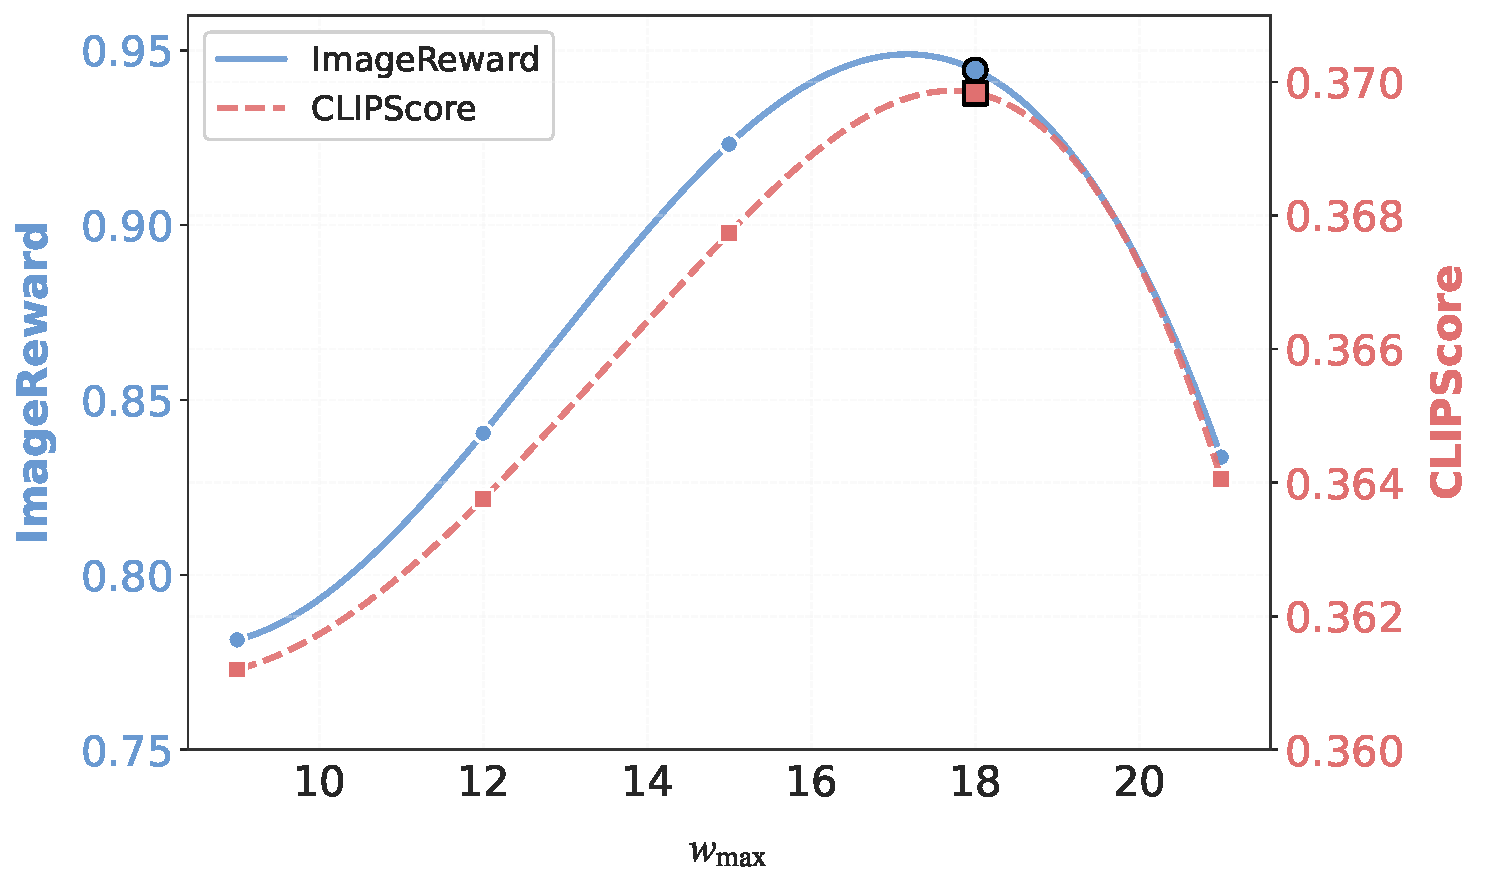
\includegraphics[width=\linewidth]{fig_tab/wmax_combined.pdf}
%         \captionsetup{justification=justified, singlelinecheck=true}
%         \caption{Ablation studies on $w_{\max}$.}
%         \label{subfig:wmax}
%     \end{subfigure}
%     \hfill 
%     \begin{subfigure}{0.49\textwidth}
%         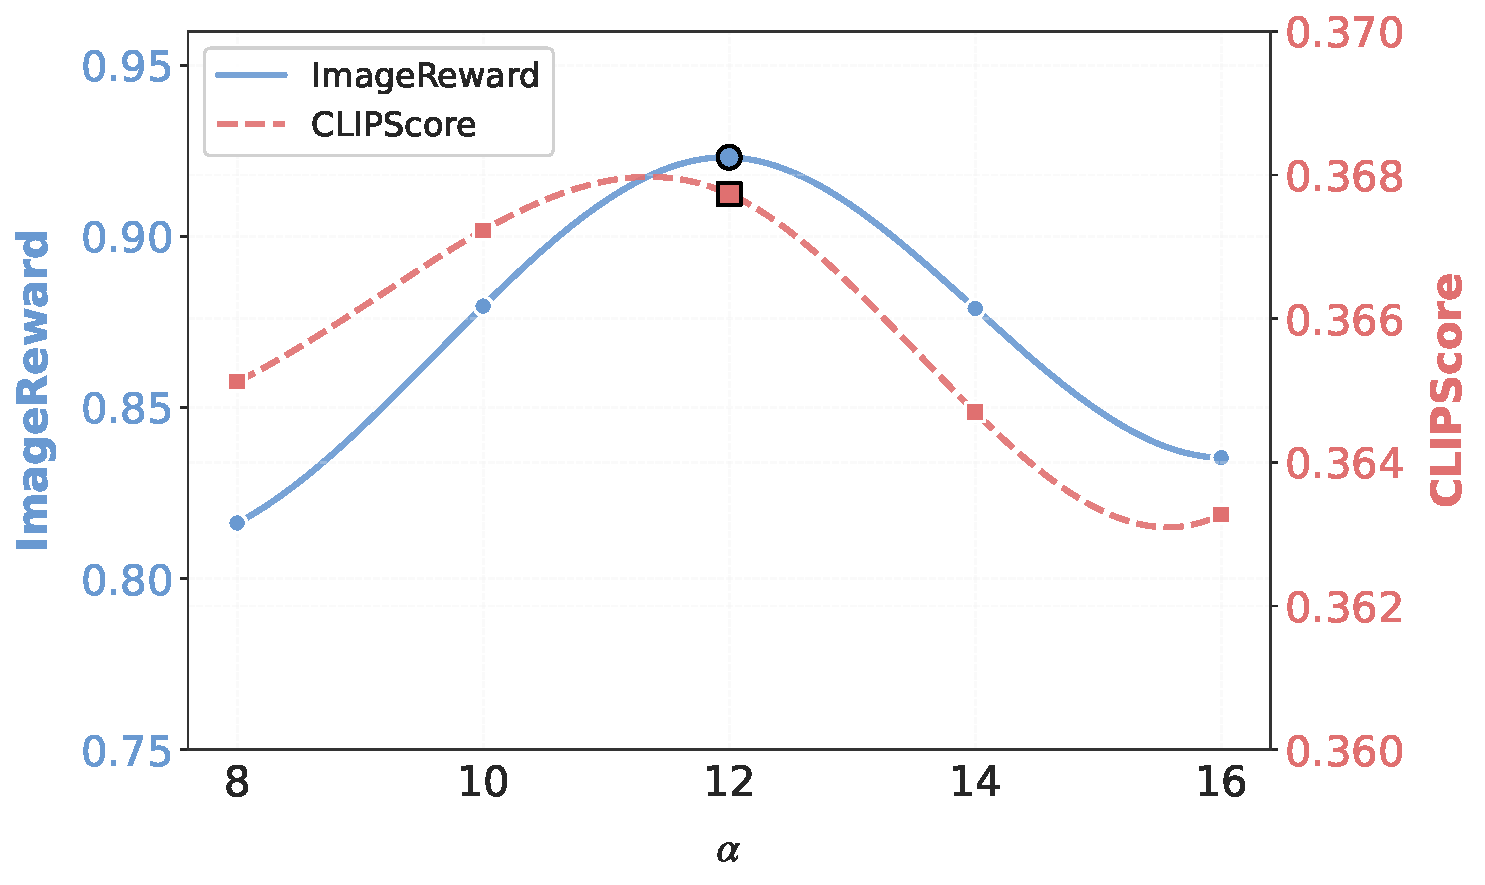
\includegraphics[width=\linewidth]{fig_tab/alpha_combined.pdf}
%         \captionsetup{justification=justified, singlelinecheck=true}
%         \caption{Ablation studies on $\alpha$.}
%         \label{subfig:alpha}
%     \end{subfigure}
%     \captionsetup{justification=justified, singlelinecheck=false}
%     \caption{Ablation studies on hyperparameters $w_{\max}$ and $\alpha$. \Cref{subfig:wmax,subfig:alpha} present the variation trends of ImageReward and CLIPScore with respect to hyperparameters and validate our optimal selection of $w_{\max}$ and $\alpha$, indicating that the generation quality of \methodabbr is largely insensitive to hyperparameter selection, with performance sustained across an extensive parameter space.}
%     \label{fig:hyper_ablation}
% \end{figure*}
\subsection{Text-to-Image Generation}
\label{subsec:txt2img_generation}
% \begin{figure*}[h]
%     \centering
%     \begin{subfigure}{0.49\textwidth}
%         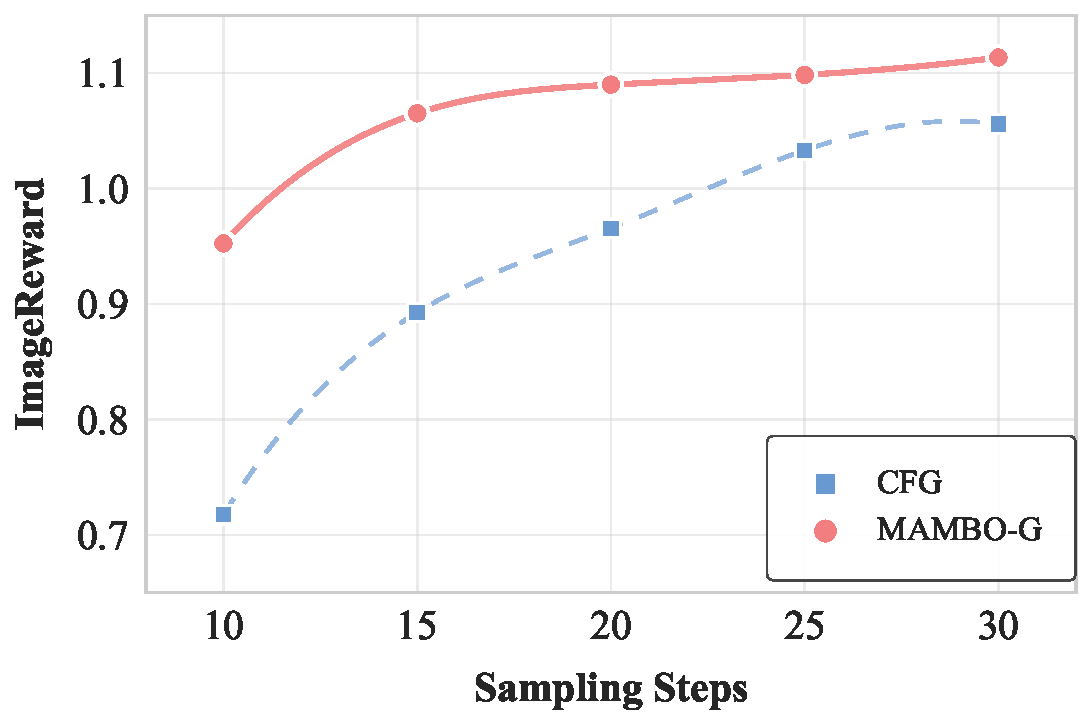
\includegraphics[width=\linewidth]{fig_tab/SD35_UniPC_ImageReward_comparison.pdf}
%         \captionsetup{justification=justified, singlelinecheck=true}
%         \caption{SD35 UniPC, ImageReward.}
%         \label{fig:sub1_1}
%     \end{subfigure}
%     \hfill
%     \begin{subfigure}{0.49\textwidth}
%         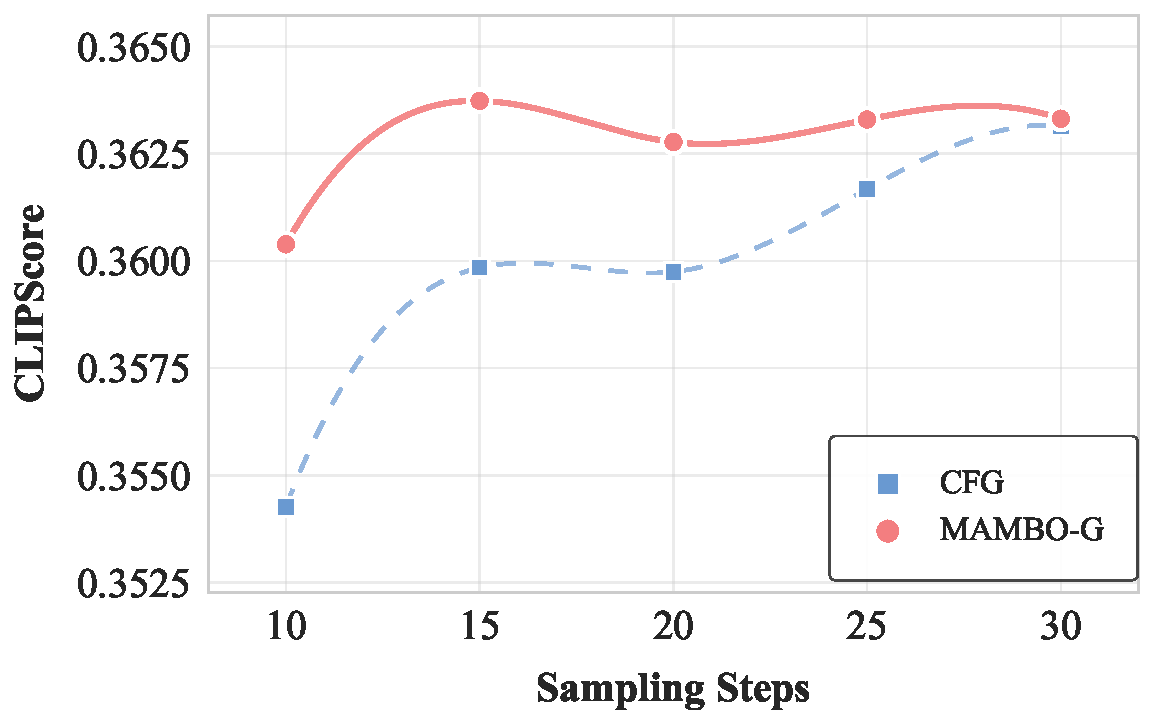
\includegraphics[width=\linewidth]{fig_tab/SD35_UniPC_CLIPScore_comparison.pdf}
%         \captionsetup{justification=justified, singlelinecheck=true}
%         \caption{SD35 UniPC, CLIPScore.}
%         \label{fig:sub1_2}
%     \end{subfigure}
%     \captionsetup{justification=justified, singlelinecheck=false}
%     \caption{Ablation studies of schedulers on UniPC. The comparative results present the consistent superiority of \mtdbk over CFG across different schedulers, further validating the wide-ranging adaptability of our method.}
%     \label{fig:unipc_ablation}
% \end{figure*}

We test \mtdbk on text-to-image generation using two recent models: Stable Diffusion v3.5 (SD3.5) and Lumina-Next (see \Cref{fig:txt2img_compare}). We measure quality with ImageReward and CLIPScore, comparing against the base samplers.
Across both models, \mtdbk improves image quality and semantic alignment. With fewer sampling steps, \mtdbk matches or exceeds longer-step baselines, speeding up generation without changing the underlying sampler.
We measure its improvement by FID as well (see \Cref{app:exp_fid}).

\subsection{Text-to-Video Generation}

We apply \mtdbk to video diffusion models and evaluate on vBench metrics for visual quality and aesthetics (see \Cref{fig:txt2video_compare}). Compared with the original guidance schedules, models with \mtdbk produce videos with higher quality and better semantic alignment at the same step count. In some cases, a smaller backbone with \mtdbk matches the quality of a larger baseline.

\subsection{Impact of Dimensionality}
\label{subsec:dim_analysis}

% \begin{table}[h]
%     \centering
%     \caption{Quantitative results of text-to-image generation across different resolutions measured by \textbf{ImageReward}. \mtdbk demonstrates consistent performance, whereas CFG degrades significantly at higher resolutions.}
%     \label{tab:resolution_ir}
%     \begin{tabular}{lcccc}
%         \toprule
%         Method & $256\times256$ & $512\times512$ & $768\times768$ & $1024\times1024$\\
%         \midrule
%         CFG & 0.53 & 0.63 & 0.30 & 0.20 \\
%         \mtdbk & \textbf{0.83} & \textbf{1.10} & \textbf{1.07} & \textbf{1.02} \\
%         \bottomrule
%     \end{tabular}
% \end{table}

\begin{table}[h]
    \centering
    \caption{\textbf{Quantitative results of text-to-image generation across different resolutions measured by \textbf{ImageReward}.} \mtdbk demonstrates consistent performance, whereas CFG degrades significantly at higher resolutions.}
    \label{tab:resolution_ir}
    \small % 略微缩小字体以增强精致感
    \begin{tabular}{ccc}
        \toprule
        Resolution & CFG (Baseline) & \textbf{\mtdbk (Ours)} \\
        \midrule
        $256 \times 256$   & 0.53 & \textbf{0.83} \\
        $512 \times 512$   & 0.63 & \textbf{1.10} \\
        $768 \times 768$   & 0.30 & \textbf{1.07} \\
        $1024 \times 1024$ & 0.20 & \textbf{1.02} \\
        \bottomrule
    \end{tabular}
\end{table}


To verify that guidance instability increases with dimensionality, we evaluate \mtdbk across different resolutions using Qwen-Image, ranging from $256\times256$ to $1024\times1024$.

We compare the ImageReward of the baseline guidance against \mtdbk. As shown in \Cref{tab:resolution_ir}, the performance gap widens significantly as resolution increases. At lower resolutions, the baseline performs adequately, and the gain from \mtdbk is marginal. However, at $1024\times1024$, the baseline frequently suffers from over-saturation and artifacts, whereas \mtdbk maintains structural coherence (see \Cref{fig:resolution_comparison_4rows}). This trend confirms that the risk of unscaled guidance updates is inherently linked to the total noise magnitude in high-dimensional spaces, making our method particularly vital for future high-resolution video models.

\subsection{Compatibility with Advanced Guidance Strategies}
\label{subsec:orthogonality}
\begin{table}[h]
    \centering
    \caption{\textbf{Orthogonality analysis of \mtdbk with other methods.} The results show that \mtdbk can be seamlessly integrated with other methods like APG \cite{sadat2024eliminating} and Rescale \cite{lin2024common} to further improve performance.}
    \label{tab:orthogonality}
    \begin{tabular}{lc}
        \toprule
        Method & ImageReward \\
        \midrule
        Baseline (Constant CFG) & 0.12 \\
        \midrule
        Rescale & 0.73 \\
        Rescale + \mtdbk & \textbf{1.12} \\
        \midrule
        APG & 0.85 \\
        APG + \mtdbk & \textbf{0.96} \\
        \bottomrule
    \end{tabular}
\end{table}
A key advantage of \mtdbk is its orthogonality to other guidance optimization
techniques. Since our method exclusively modulates the guidance scale, it can be directly stacked with methods that normalize the update vector or alter the sampling trajectory.

To verify this, we evaluate \mtdbk in combination with Guidance Rescale (GR)~\cite{lin2024common} and Adaptive Projection Guidance (APG) using the Qwen-Image model. GR rescales the guidance vector to prevent over-exposure, while APG dynamically adjusts the projection direction. As shown in our comparisons (\Cref{tab:orthogonality}), while both baselines effectively mitigate some artifacts, stacking them with \mtdbk yields further consistent improvements in ImageReward. This plug-and-play nature ensures \mtdbk remains relevant even as new guidance strategies are developed.


\subsection{Ablation Studies and Hyperparameters}
\label{subsec:ablation}

We perform ablation studies to understand the impact of our modeling choices.

\textbf{Guidance schedule.} We compare several ways of mapping $r_t$ to a guidance scale, including exponential decay, linear decay, and simple inverse functions. Exponential decay provides a good balance between stability and detail in our experiments (see \Cref{fig:function_ablation}), so we use it as the default.

\begin{table}[h]
    \centering
    \caption{\textbf{Comparison with time-based schedule on Qwen-Image (10 steps).} The time-based schedule uses the average guidance scale of \mtdbk at each step. The results highlight the importance of instance-level adaptation.}
    \label{tab:time_vs_instance}
    \begin{tabular}{lc}
        \toprule
        Method & ImageReward \\
        \midrule
        Baseline (Constant CFG) & 0.12 \\
        Time-based Schedule & 0.83 \\
        \mtdbk (Ours) & \textbf{1.08} \\
        \bottomrule
    \end{tabular}
\end{table}

\textbf{Instance-aware vs. Time-based Schedule.} A natural question is whether a simple time-dependent schedule suffices. To investigate this, we constructed a ``Time-based Schedule'' baseline by averaging the effective guidance scale $w(r_t)$ of \mtdbk across all samples at each timestep, then applying this fixed curve to all generated images. As shown in \Cref{tab:time_vs_instance}, the time-based schedule significantly improves over the constant baseline (ImageReward $0.12 \to 0.83$), confirming that dampening early-stage guidance is generally beneficial. However, \mtdbk achieves a further substantial improvement ($0.83 \to 1.08$). This gap underscores the critical role of \textit{instance-awareness}: since instability varies across random seeds, a fixed schedule over-penalizes stable samples or under-penalizes risky ones, whereas \mtdbk adapts dynamically.

\textbf{Hyperparameter sensitivity.} We vary $w_{\max}$ and the decay rate $\alpha$ over a range of values (see \Cref{tab:wmax_ablation,tab:alpha_ablation}). \mtdbk maintains stable behavior and competitive scores across a broad region, suggesting it does not require heavy tuning.

\textbf{Scheduler generalization.} We also apply \mtdbk on ODE solvers such as UniPC (see \Cref{fig:unipc_ablation}). The method still improves over the corresponding baselines, showing it can be combined with different samplers.

% These experiments validate our design. Despite its simplicity, MAMBO-G is effective and integrates cleanly with existing diffusion and flow-based generators.


